\documentclass[9pt]{beamer}
\usepackage{beamerthemeshadow}
\usepackage{graphicx}
\usepackage{color}
\usepackage[utf8]{inputenc}
\usepackage{hyperref}
\usepackage{setspace}
\usepackage[T1]{fontenc}
\usepackage[flushleft]{threeparttable}
\definecolor{beamer@darkred}{rgb}{0.4,0.15,0.75}
\setbeamercolor{structure}{fg=beamer@darkred}



\def\d{{\fontencoding{T1}\selectfont\dj}}
\def\D{{\fontencoding{T1}\selectfont\DJ}}



\title{Tehničko i naučno pisanje}
\subtitle{Proširena stvarnost i mogćnosti njene primene u obrazovanju}
\author{Matija Đorđević  Filip Nedeljković\\
Mlađan Simić  Igor Stojanović}
\institute{Matematički fakultet\\Univerzitet u Beogradu}
\date{
	\footnotesize{Beograd, 2022.}	
}

\begin{document}

\begin{frame}
	\thispagestyle{empty}
	\titlepage
\end{frame}

\addtocounter{framenumber}{-1}







\begin{frame}
	\frametitle{Pregled} % Table of contents slide, comment this block out to remove it
	\tableofcontents[hidesubsections] 
\end{frame}

\section{Uvod}

\begin{frame}[fragile]\frametitle{Uvod}
	\begin{itemize}	
 \setlength\itemsep{1.5em}
		\item Proširena stvarnost - spoj fizičkog i digitalnog sveta, u kojem digitalni elementi dopunjavaju fizički svet
		\item Razlika između AR i VR - VR zamenjuje stvarni svet, dok AR dodaje informacije stvarnom svetu
		\item S obzirom na bogato okruženje za učenje koje nudi AR, istaknuta je i primena ove tehnologije u oblasti obrazovanja.
	
	\end{itemize}
\end{frame}


\section{Istorija}
	\begin{frame}
    \frametitle{Istorija}
        \begin{itemize}
            \setlength\itemsep{1.5em}
            \item Iako je pojam zaživeo u skorije vreme, ljudi su se stotinama godina bavili proširenom realnošću koristeći optičku nauku.
            \item Nakon Drugog svetskog rata, centar razvoja proširene realnosti postaju SAD. Zahvaljujući napretku računara stvaraju se nove mogućnosti za inovaciju.
            \item Sa završetkom Hladnog rata, otvara se mogućnost za upotrebu ove tehnologije izvan vojno-industrijske svrhe.
            \item Danas, mobilni uređaji imaju glavnu ulogu u razvoju proširene realnosti.
		\end{itemize}
	\end{frame}
	
\section{Način rada AR tehnologija}
\subsection{Hardver}
	\begin{frame}
 \frametitle{Hardver}
        \begin{itemize}
            \setlength\itemsep{1.5em}
                \item Osnovne tri hardverske komponente su: senzor, procesor i displej.
                \item Senzori – Njihova uloga, povezanost sa procesorom i najkorišćenije vrste senzora: kamera, mikrofon, elektromagnetno praćenje i mehaničko 			praćenje.
                \item Procesor – Uloga procesora u radu, povezanost sa displejom i ograničenost procesora zbog drugih komponenata.
                \item Displej – Način rada i vrste vizualnih displeja koji se najčešće koriste.
        \end{itemize}
            
	\end{frame}

\subsection{Softver}
	\begin{frame}
 \frametitle{Softver}
        \begin{itemize}
            \setlength\itemsep{1.5em}
                \item Kategorija softvera potrebnih za pravljenje AR:
                \begin{itemize}
                \setlength\itemsep{1.5em}
                    \item softver direktno u AR aplikaciji
                    \begin{itemize}
                        \item Environmental Acquisition softver 
                        \item softver za renderovanje
                        \item Application engine
                    \end{itemize}
                    \item softver za pravljenje AR aplikacije
                    \item softver za pravljenje sadrˇzaja AR aplikacije
                \end{itemize}
        \end{itemize}
            
	\end{frame}
 
\section{Primena u obrazovanju}
\subsection{Primena AR  tehnologije u obrazovanju}
	\begin{frame} 
 \frametitle{Primena AR  tehnologije u obrazovanju}
    \begin{itemize}
    \setlength\itemsep{1.5em}
            \item AR i VR se koriste zbog visoke interaktivnosti i sposobnosti predstavljanja virtuelnog okruženja koje podseća na stvarni svet
            \item Istraživanja potvrđuju da tehnološki alati pomažu pri učenju
            \item Moguće je istraživanje i manipulisanje trodimenzionalnim interaktivnim okruženjem 
    \end{itemize}
 
	\end{frame}



 
\subsection{Primeri mogućnosti primene}

 \begin{frame}
 \frametitle{Primeri mogućnosti primene}
            \begin{itemize}
            \setlength\itemsep{1.5em}
		\item Postoje aplikacije koje olakšavaju učenicima da razumeju bolje prostorno okruženje. 
            \end{itemize}
            \begin{figure}[h!]
		\begin{center}
		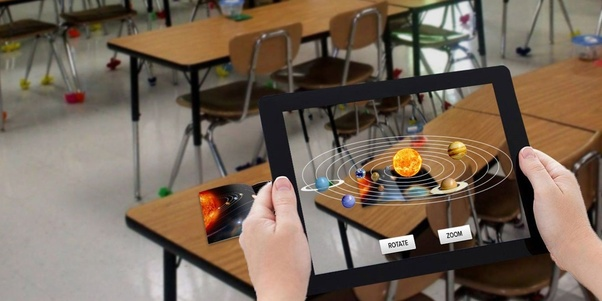
\includegraphics[scale=0.3]{primer.jpg}
		\end{center}
  \begin{itemize}
		\item Proširena stvarnost se može koristiti i kao pomoćno sredstvo u radu sa učenicima koji imaju smetnje u razvoju.
            \end{itemize}
		
		\end{figure}
\end{frame}
\section{Zakljucak}

\begin{frame}[fragile]\frametitle{Zaključak}
	
		\begin{itemize}
  \setlength\itemsep{1.5em}
			\item VR i AR se sve više primenjuje u okviru obrazovnih procesa i njihov potencijal umnogome doprinosi studentima
			\item Ono što se izdvaja kao zajedničko jeste:
   
   \begin{itemize}
   \item mogućnost neposredne interakcije sa fizički nedostupnim objektima 
    \item upoznavanje sa predmetima i situacijama na interesantan i razumljiv način
   
\end{itemize}

  
		\end{itemize}

\end{frame}

\end{document}
